\documentclass[12pt]{report}

\usepackage{natbib}
\usepackage{graphicx}
\usepackage{lipsum}
\usepackage[bookmarks=false, colorlinks=true, citecolor=blue, linkcolor=blue]{hyperref}

\usepackage[a4paper,left=2.5cm,right=2.5cm,top=2.5cm,bottom=2.5cm]{geometry}
\usepackage{fancyhdr}
\usepackage{datetime}
\usepackage{diagbox}

\usepackage[listings]{tcolorbox}

\newtcblisting{commandshell}{colback=white,colupper=black,colframe=black!25, listing only}
\newtcblisting{textfile}{colback=yellow!3!white,colupper=black,colframe=black!25, listing only}

\pagestyle{fancy}

\renewcommand{\chaptermark}[1]{\markboth{\MakeUppercase{\chaptername\ #1}}{}}

\renewcommand{\chaptername}{}

\usepackage{titlesec}
\titleformat{\chapter}[hang]{\bfseries\huge}{}{0ex}{\thechapter.~}[]
\titleformat{name=\chapter,numberless}[hang]{\bfseries\huge}{}{0ex}{}[]
\titleformat{\section}[block]{\bfseries\Large}{}{0ex}{\thesection~}[]
\titleformat{name=\section,numberless}[block]{\bfseries\Large}{}{0ex}{}[]
\titleformat{\subsection}[block]{\bfseries\large}{}{0ex}{\thesubsection~}[]
\titleformat{name=\subsection,numberless}[block]{\bfseries\large}{}{0ex}{}[]



\def\mydate{\leavevmode\hbox{\the\day~\monthname, \the\year}}
\def\twodigits#1{\ifnum#1<10 0\fi\the#1}

% Standard journal abbreviations
% Mostly as used by ADS, with a few additions for journals where MNRAS does not
% follow normal IAU style.

\newcommand\aap{A\&A}                % Astronomy and Astrophysics
\let\astap=\aap                          % alternative shortcut
\newcommand\aapr{A\&ARv}             % Astronomy and Astrophysics Review (the)
\newcommand\aaps{A\&AS}              % Astronomy and Astrophysics Supplement Series
\newcommand\actaa{Acta Astron.}      % Acta Astronomica
\newcommand\afz{Afz}                 % Astrofizika
\newcommand\aj{AJ}                   % Astronomical Journal (the)
\newcommand\ao{Appl. Opt.}           % Applied Optics
\let\applopt=\ao                         % alternative shortcut
\newcommand\aplett{Astrophys.~Lett.} % Astrophysics Letters
\newcommand\apj{ApJ}                 % Astrophysical Journal
\newcommand\apjl{ApJ}                % Astrophysical Journal, Letters
\let\apjlett=\apjl                       % alternative shortcut
\newcommand\apjs{ApJS}               % Astrophysical Journal, Supplement
\let\apjsupp=\apjs                       % alternative shortcut
% The following journal does not appear to exist! Disabled.
%\newcommand\apspr{Astrophys.~Space~Phys.~Res.} % Astrophysics Space Physics Research
\newcommand\apss{Ap\&SS}             % Astrophysics and Space Science
\newcommand\araa{ARA\&A}             % Annual Review of Astronomy and Astrophysics
\newcommand\arep{Astron. Rep.}       % Astronomy Reports
\newcommand\aspc{ASP Conf. Ser.}     % ASP Conference Series
\newcommand\azh{Azh}                 % Astronomicheskii Zhurnal
\newcommand\baas{BAAS}               % Bulletin of the American Astronomical Society
\newcommand\bac{Bull. Astron. Inst. Czechoslovakia} % Bulletin of the Astronomical Institutes of Czechoslovakia 
\newcommand\bain{Bull. Astron. Inst. Netherlands} % Bulletin Astronomical Institute of the Netherlands
\newcommand\caa{Chinese Astron. Astrophys.} % Chinese Astronomy and Astrophysics
\newcommand\cjaa{Chinese J.~Astron. Astrophys.} % Chinese Journal of Astronomy and Astrophysics
\newcommand\fcp{Fundamentals Cosmic Phys.}  % Fundamentals of Cosmic Physics
\newcommand\gca{Geochimica Cosmochimica Acta}   % Geochimica Cosmochimica Acta
\newcommand\grl{Geophys. Res. Lett.} % Geophysics Research Letters
\newcommand\iaucirc{IAU~Circ.}       % IAU Cirulars
\newcommand\icarus{Icarus}           % Icarus
\newcommand\japa{J.~Astrophys. Astron.} % Journal of Astrophysics and Astronomy
\newcommand\jcap{J.~Cosmology Astropart. Phys.} % Journal of Cosmology and Astroparticle Physics
\newcommand\jcp{J.~Chem.~Phys.}      % Journal of Chemical Physics
\newcommand\jgr{J.~Geophys.~Res.}    % Journal of Geophysics Research
\newcommand\jqsrt{J.~Quant. Spectrosc. Radiative Transfer} % Journal of Quantitiative Spectroscopy and Radiative Transfer
\newcommand\jrasc{J.~R.~Astron. Soc. Canada} % Journal of the RAS of Canada
\newcommand\memras{Mem.~RAS}         % Memoirs of the RAS
\newcommand\memsai{Mem. Soc. Astron. Italiana} % Memoire della Societa Astronomica Italiana
\newcommand\mnassa{MNASSA}           % Monthly Notes of the Astronomical Society of Southern Africa
\newcommand\mnras{MNRAS}             % Monthly Notices of the Royal Astronomical Society
\newcommand\na{New~Astron.}          % New Astronomy
\newcommand\nar{New~Astron.~Rev.}    % New Astronomy Review
\newcommand\nat{Nature}              % Nature
\newcommand\nphysa{Nuclear Phys.~A}  % Nuclear Physics A
\newcommand\pra{Phys. Rev.~A}        % Physical Review A: General Physics
\newcommand\prb{Phys. Rev.~B}        % Physical Review B: Solid State
\newcommand\prc{Phys. Rev.~C}        % Physical Review C
\newcommand\prd{Phys. Rev.~D}        % Physical Review D
\newcommand\pre{Phys. Rev.~E}        % Physical Review E
\newcommand\prl{Phys. Rev.~Lett.}    % Physical Review Letters
\newcommand\pasa{Publ. Astron. Soc. Australia}  % Publications of the Astronomical Society of Australia
\newcommand\pasp{PASP}               % Publications of the Astronomical Society of the Pacific
\newcommand\pasj{PASJ}               % Publications of the Astronomical Society of Japan
\newcommand\physrep{Phys.~Rep.}      % Physics Reports
\newcommand\physscr{Phys.~Scr.}      % Physica Scripta
\newcommand\planss{Planet. Space~Sci.} % Planetary Space Science
\newcommand\procspie{Proc.~SPIE}     % Proceedings of the Society of Photo-Optical Instrumentation Engineers
\newcommand\rmxaa{Rev. Mex. Astron. Astrofis.} % Revista Mexicana de Astronomia y Astrofisica
\newcommand\qjras{QJRAS}             % Quarterly Journal of the RAS
\newcommand\sci{Science}             % Science
\newcommand\skytel{Sky \& Telesc.}   % Sky and Telescope
\newcommand\solphys{Sol.~Phys.}      % Solar Physics
\newcommand\sovast{Soviet~Ast.}      % Soviet Astronomy (aka Astronomy Reports)
\newcommand\ssr{Space Sci. Rev.}     % Space Science Reviews
\newcommand\zap{Z.~Astrophys.}       % Zeitschrift fuer Astrophysik


\begin{document}

\begin{titlepage}

\vspace*{4cm}
\begin{center}

{\fontfamily{cmss}\selectfont
\Huge
\textbf{
HSIM Manual\\[0.5ex]
\Large
v311}
\vspace{2cm}

\large
\mydate
}
\end{center}
\vspace*{\fill}


\end{titlepage}

\tableofcontents

\vfill
\subsection*{Revision History}

\begin{table*}[h]
\label{tab:revision}
\begin{tabular}{lll}
\hline
Version & Date & Comments \\
\hline
1.0 & 2018-09-27 & HSIM v204 release \\
1.1 & --- & HSIM v210 release \\
1.2 & 2019-03-28 & HSIM v211 release \\
1.2b & 2019-04-30 & HSIM v212 release \\
1.3 & 2019-10-11 & Detector systematics \\
1.3b & 2019-10-16 & HSIM v300 release \\
1.4 & 2019-12-16 & HSIM v302 release \\
1.5 & 2020-04-21 & HSIM v303 release \\
1.6 & 2021-06-01 & HSIM v310 release \\
1.7 & & HSIM v311 release \\
\hline
\end{tabular}
\end{table*}


\subsection*{Authors of this document}
Miguel Pereira Santaella (CAB) \\
Laurence Routledge (University of Oxford)

\clearpage

\chapter{Quick Start Guide}

\section{Introduction and Installation}

HSIM is a dedicated pipeline for simulating observations with HARMONI on the Extremely Large Telescope. HSIM takes high spectral and spatial resolution input data cubes, encoding physical descriptions of astrophysical sources, and generates mock observed data cubes. The simulations incorporate detailed models of the sky, telescope, instrument, and detectors to produce realistic mock data \citep{Zieleniewski2015}.

HSIM is programmed in Python3 and the source code can be found at \url{https://github.com/HARMONI-ELT/HSIM}. It does not require any installation, just clone the GitHub repository 

\begin{commandshell}
$ git clone https://github.com/HARMONI-ELT/HSIM.git
\end{commandshell}

HSIM depends on the following Python packages to work:

\begin{itemize}
\setlength\itemsep{-0.5ex}
\item astropy 4.1
\item numpy 1.19.5
\item scipy 1.5.4
\item matplotlib 3.3.4
\item photutils 0.7
\end{itemize}

The code has been tested with the indicated package version, although more recent releases of these packages are likely to work as well.


\section{Running Simulations}

\subsection{Preparing the Input Datacube}

Before running HSIM, you will need an input model of your astronomical object stored as a datacube in a \textsc{fits} file. The recommended sizes for the spatial pixels (spaxels) are 0.8, 2, 4, or 6 mas depending on the selected spaxel scale for HARMONI (see Table~\ref{tab:scale}). If your datacube has a different spaxel scale, HSIM will automatically interpolate\slash rebin the input datacube to the recommended values.

\begin{table*}[h]
\centering
\caption{Recommended input pixel size}
\label{tab:scale}
\begin{tabular}{cccc}
\hline
HARMONI & Recommended\\
Spaxel scale & input scale\\
(mas) & (mas) \\
\hline
4$\times$4   & 0.8 \\
10$\times$10 & 2.0 \\
20$\times$20 & 4.0 \\
30$\times$60, 60$\times$60, 120$\times$60 & 6.0 \\
\hline
\end{tabular}
\end{table*}

Similarly, it is recommended to oversample the spectral dimension of the input cube by a factor of 4 with respect to the nominal resolving power ($R$) of the selected grating (e.g., the spectral sampling for the K-grating $R$=7100 at 2.2$\mu$m should be 0.078\,nm). If your input cube has a different spectral sampling, HSIM will interpolate\slash rebin it. 

The information on the spatial and spectral sampling of the input cube are passed through the \textsc{fits} file header to HSIM (Table~\ref{tab:fits_header} shows a summary of all the header keywords used by HSIM). In particular, the \texttt{CDELT1} and \texttt{CDELT2} header values are used to get the spatial scale, and \texttt{CDELT3} to obtain the spectral sampling. The spectral resolution of the input cube is indicated by \texttt{SPECRES} in wavelength units similar to \texttt{CDELT3}. The units of these values are those indicated by the \texttt{CUNIT1}, \texttt{CUNIT2}, and \texttt{CUNIT3} header values. For the spatial units (\texttt{CUNIT1} and \texttt{CUNIT2}), the accepted values are any angular units supported by astropy (e.g., \texttt{mas}, \texttt{arcsec}). For the spectral units, \texttt{CUNIT3} and \texttt{SPECRES}, HSIM recognizes any length unit supported by astropy (e.g., \texttt{angstrom}, \texttt{nm}, \texttt{micron}). The size of the input cube is obtained from \texttt{NAXIS1}, \texttt{NAXIS2}, and \texttt{NAXIS3}.


The wavelength of each slice of the data cube are also calculated from the \textsc{fits} header using the following relation:
\begin{equation}\label{eq:lambda}
\lambda_i = \texttt{CRVAL3} + \texttt{CDELT3} \times (i - \texttt{CRPIX3})
\end{equation}

where $i$ is the slice number from 1 to $\texttt{NAXIS3}$. The wavelength range of the input cube and the selected grating should, at least, partially overlap.

Finally, the input data cube should be in surface brightness units indicated by \texttt{BUNIT}. The accepted values are any surface spectral flux density units supported by astropy (e.g., \texttt{erg/s/cm2/um/arcsec2}, \texttt{erg/s/cm2/AA/arcsec2}, \texttt{MJy/sr}).


\begin{table*}[h]
\footnotesize
\centering
\caption{\textsc{fits} header keywords used by HSIM}
\label{tab:fits_header}
\begin{tabular}{lp{75mm}p{50mm}}
\hline
Keyword & Description & Accepted values \\
\hline
\multicolumn{3}{c}{Spatial information}\\
\hline
NAXIS\{1,2\} & Number of pixels along x-axis and y-axis\\
CTYPE1 & Type of the spatial x-axis & x, ra, RA-{}-{}-SIN, RA-{}-{}-TAN \\
CTYPE2 & Type of the spatial y-axis & y, dec, DEC-{}-SIN, DEC-{}-TAN \\
CDELT\{1,2\} & X and Y pixel size \\
CUNIT\{1,2\} & Units of CDELT\{1,2\} & any angular unit supported by astropy (e.g., mas, arcsec)\\
\hline
\multicolumn{3}{c}{Spectral information}\\
\hline
NAXIS3 & Number of spectral pixels \\
CTYPE3 & Type of the spectral axis & wavelength \\
CDELT3 & Size of the spectral pixel \\
SPECRES & Spectral resolution in wavelength units &  \\
CRPIX3 & Reference pixel for the spectral axis (see Equation~\ref{eq:lambda}) \\
CRVAL3 & Wavelength of the reference pixel\\
CUNIT3 & Units of CDELT3, CRVAL3, and SPECRES & any length unit supported by astropy (e.g., angstrom, AA, nm, micron) \\
\hline
\multicolumn{3}{c}{Flux units}\\
\hline
BUNIT & Flux units of the cube & any surface spectral flux density unit supported by astropy (e.g., erg/s/cm2/um/arcsec2, erg/s/cm2/AA/arcsec2, MJy/sr) \\
\hline
\end{tabular}
\end{table*}


\subsection{HSIM Gratings}

The gratings that can be selected in HSIM are detailed below in Table~\ref{tab:gratings}.
\begin{table*}[!h]
\centering
\caption{HSIM grating parameters}
\label{tab:gratings}
\begin{tabular}{lccc}
\hline
Grating & $\lambda_{min}$ ($\mu$m) & $\lambda_{max}$ ($\mu$m) & R \\
\hline
\multicolumn{4}{c}{Low resolution}\\
\hline
V+R & 0.458 & 0.820 & 3100 \\
Iz+J & 0.811 & 1.369 & 3355 \\
H+K & 1.450 & 2.450 & 3355 \\
\hline
\multicolumn{4}{c}{Medium resolution}\\
\hline
Iz & 0.830 & 1.050 & 7104 \\
J & 1.046 & 1.324 & 7104 \\
H & 1.435 & 1.815 & 7104 \\
K & 1.951 & 2.469 & 7104\\
\hline
\multicolumn{4}{c}{High resolution}\\
\hline
z-high & 0.828 & 0.902 & 17385 \\
J-short & 1.012 & 1.102 & 17385 \\
J-long & 1.098 & 1.189 & 17385 \\
H-high & 1.538 & 1.678 & 17385 \\
K-short & 2.017 & 2.201 & 17385 \\
K-long & 2.199 & 2.400 & 17385 \\
\hline
\end{tabular}
\end{table*}

\subsection{Detector Systematics}

If chosen, HSIM can be run with more detailed detector systematics to simulate some of the features seen on infra-red detectors. When this option is selected, HSIM creates 8 simulated HAWAII 4RGs where each pixel has a unique read noise value derived from analysing the KMOS H2RG detectors. The read noise values have a distribution, with the peak at the expected read noise value for the H4RGs. An example HSIM H4RG is seen in Figure~\ref{fig:hsimdet}. This also utilises the HXRG noise generation tool provided by Teledyne~\citep{Rauscher2015} to add additional features, such as ACN and amplifier bias differences. The parameters of these have been tuned to an expected performance level, however can be adjusted in the config file.  Additionally, in the config file there is an option to use a different read noise file, by changing the \texttt{rn\_file} to point to a different \textsc{fits} file. This file determines the distribution the read noise will follow, so adding a file with a uniform value across the image will produce a flat distribution. The last detector systematics option, \texttt{force\_new}, determines whether or not to generate a new set of detectors with each simulation. By default, the first time you run detailed detector systematics, it will save the read noise maps generated to a location specified when initialising HSIM, and use these in subsequent runs of the code to speed up the simulation. New shot noise will still be generated each time. If desired however, new detectors can be made each time, either by setting this parameter to False, or by manually deleting the created \texttt{HARMONI\_dets.fits} file in the location in which they are saved.

\begin{figure*}[!h]
\centering
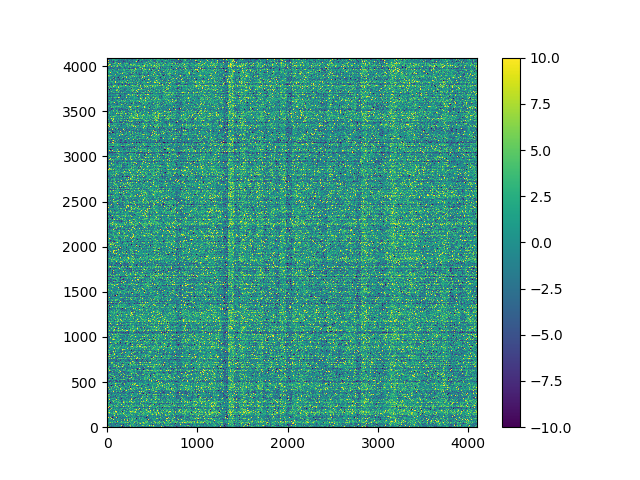
\includegraphics[width=\textwidth]{hsim-sim-det.png}
\caption{\small HSIM simulated detector.}\label{fig:hsimdet}
\end{figure*}

The simulated data cube is then sliced up and added to these detectors, in a manner similar to the effect of the image slicer. This ensures that features that appear linear on the detectors no longer appear linear in the output data cube. The simulation is then folded back into a standard data cube to maintain the `cube in, cube out' nature of HSIM. When creating the reduced cube, a separate instance of the detectors is generated and used in the reduction, so the residual features will remain in the reduced cube. A separate cube is returned containing the detectors used in the simulation.

\subsection{Running HSIM}

Once the input data cube has been prepared, the next step is to run HSIM. HSIM comes with a graphical user interface (GUI) which can be used to define the input parameters of the simulations. Alternatively, the same options can be accessed from a configuration file or directly from the command line.

\subsubsection{GUI}

The GUI provides a relatively easy way to list the available options. To launch HSIM in the GUI mode, type the following command\\

\begin{commandshell}
$ python3 hsim3.py
\end{commandshell}

Then, a window similar to that shown in Figure~\ref{fig:hsimgui} should appear. In that window, it is possible to select the input cube and the output directory and define all the parameters needed by HSIM to run the simulation (these parameters are explained in Section~\ref{s:list_options}). Clicking on the \texttt{Commence simulation} button will start the simulation. You can see how the simulation advances in the terminal window from where HSIM was called.

\begin{figure*}[!h]
\centering
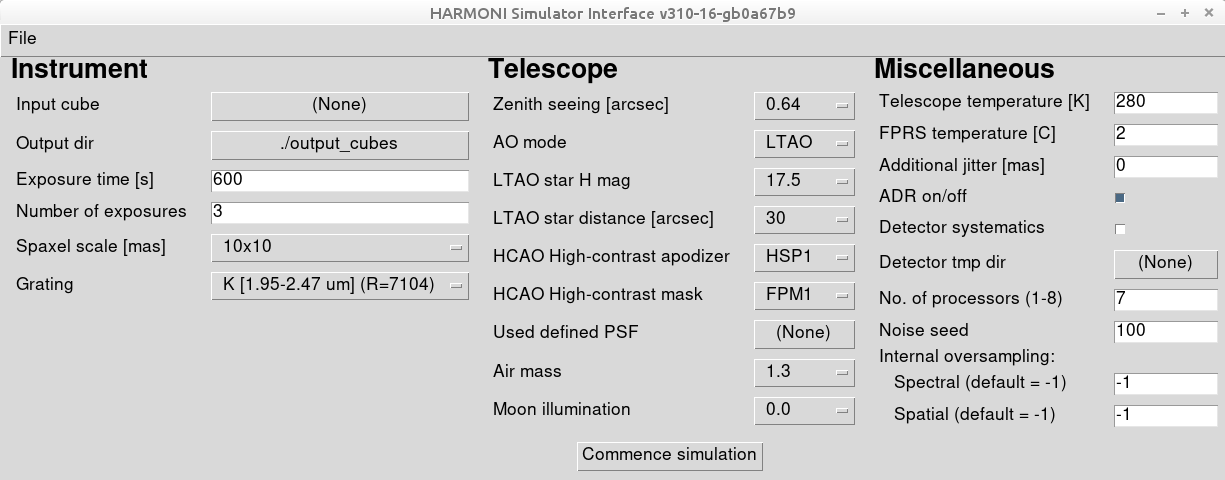
\includegraphics[width=\textwidth]{HSIM_GUI.png}
\caption{\small HSIM GUI.}\label{fig:hsimgui}
\end{figure*}

\subsubsection{Command-line}

All the GUI options can be directly accessed from the command line mode using the following command

\begin{commandshell}
$ python3 hsim3.py -b --arg1 value1 --arg2 value2 ...
\end{commandshell}

where \texttt{arg*} are the parameters of the simulation (see Section~\ref{s:list_options}). \texttt{-b} forces HSIM to start the simulation not showing the GUI. Otherwise, the parameters are read from the command line (and the configuration file if specified with \texttt{-c}, see below) and then the GUI will appear. Adding \texttt{-h} will show all the command line options and their default and accepted values.


\subsubsection{Configuration file}

It is also possible to define the simulation input parameters using a configuration file using

\begin{commandshell}
$ python3 hsim3.py -b -c config_file
\end{commandshell}

Additional input parameters can be added to the command line if required. As in the command-line case, \texttt{-b} forces HSIM to start the simulation not showing the GUI.

In the case of conflicting input parameters, preference is given to the GUI, then the command-line, and finally the configuration file.


\subsection{List of Options}\label{s:list_options}

The available HSIM options are listed below. The complete list is also available by running 
\begin{commandshell}
$ python3 hsim3.py -h
\end{commandshell}

These options are preceded by \texttt{--} when included in the command-line. When they are used in a configuration file the ``\texttt{-}'' in their names should be replaced by ``\texttt{\_}'' (see example below).

\begin{description}
% \setlength\itemsep{-0.5ex}
\item \texttt{input-cube}: Path of the \textsc{fits} input datacube.

\item \texttt{output-dir}: Output directory.

\item \texttt{grating}: HARMONI grating. Available values are: \texttt{V+R, Iz+J, H+K, Iz, J, H, K, z-high, J-short, J-long, H-high, K-short, K-long}.

\item \texttt{spaxel-scale}: HARMONI spatial scale in mas. Available values are: \texttt{4x4, 10x10, 20x20, 30x60, 60x60, 120x60}. The 60x60 and 120x60 scales are only available for the V+R grating.

\item \texttt{exposure-time}: Integration time of each exposure in seconds (e.g., \texttt{600}).

\item \texttt{n-exposures}: Number of exposures (e.g., \texttt{3}).

\item \texttt{ao-mode}: Adaptive optics mode of the observations. Available values are: \texttt{LTAO, SCAO, HCAO, noAO, Airy, User}. \texttt{LTAO} corresponds to the Laser Tomography Adaptive Optics mode, \texttt{SCAO} to the Single Conjugate Adaptive Optics mode, \texttt{HCAO} to the High Contrast Adaptive Optics mode, \texttt{noAO} indicates that no adaptive optics corrections are applied, \texttt{Airy} uses the diffraction limit of the ELT, and \texttt{User} uses the 2D user-defined PSF indicated by the parameter \texttt{user-defined-psf}.

\item \texttt{user-defined-psf}: \textsc{fits} file containing a 2D user-defined PSF.

\item \texttt{ao-star-hmag}: H magnitude of the LTAO AO star. Available values are: \texttt{15.0, 17.5, 19.0}. The default is \texttt{17.5}.

\item \texttt{ao-star-distance}: Distance from the HARMONI FoV center to the LTAO AO star in arcsec. Available values are: \texttt{15, 30, 45}. The default is \texttt{30}.

\item \texttt{hc-apodizer}: High-contrast apodizer used for the HCAO mode. Available values are: \texttt{HSP1, HSP2}. The default is \texttt{HSP1}.

\item \texttt{hc-fp-mask}: High-contrast mask used for the HCAO mode. Available values are: \texttt{FPM1}. The default is \texttt{FPM1}.

\item \texttt{zenith-seeing}: Optical (500\,nm) zenith atmospheric seeing FWHM in arcsec. Available values are: \texttt{0.43, 0.57, 0.64, 0.72, 1.04}.

\item \texttt{air-mass}: Average air mass during the HARMONI observation. Available values are: \texttt{1.1, 1.3, 1.5, 2.0}, which correspond to zenith angles of 25$^{\circ}$, 40$^{\circ}$, 48$^{\circ}$, and 60$^{\circ}$, respectively.

\item \texttt{moon-illumination}: Fraction of the Moon that is illuminated at the time of the observation. A 30$^{\circ}$ separation between target and Moon is assumed. Available values are: \texttt{0, 0.5, 1.0}. The default is \texttt{0.0}.

\item \texttt{detector-systematics}: Indicates if the detector systematics are simulated. It only affects the observed outputs (see Section~\ref{s:output}). Available values are \texttt{True, False}.

\item \texttt{detector-tmp-path}: Path of the desired location to save the created detectors if using advanced detector systematics. Use \texttt{None} to use the default location (\texttt{sim\_data/detectors}).

\item \texttt{adr}: When this option is set, the atmospheric differential refraction is first simulated and then corrected in the output cubes in a way similar to what is expected from the pipieline. If it is set to \texttt{False}, the atmospheric differential refraction and its correction are not simulated. Available values are \texttt{True, False}. The default is \texttt{True}.

\item \texttt{telescope-temp}: Temperature of the site\slash telescope in K. This is used to calculate the telescope and part of the instrument background emission. The default value is \texttt{280}.

\item \texttt{fprs-temp}: Temperature of the HARMONI Focal Plane Relay Subsystem (FPRS) in C degrees. This is used to calculate part of the instrument background emission. The default value is \texttt{-15}.

\item \texttt{extra-jitter}: Additional telescope PSF blur in mas. The default is \texttt{0}. It is possible to define independent jitter values for the each axis (e.g., \texttt{2x4}).

\item \texttt{noise-seed}: Random number generator seed using during the simulation. It only affects the observed outputs (see Section~\ref{s:output}).

\item \texttt{n-cpus}: Number of processors used by HSIM.

\item \texttt{spectral-sampling}: Internal spectral oversampling factor. If not specified, the default internal sampling is 4 times the spectral resolution of the selected grating.

\item \texttt{spatial-sampling}: Internal spatial oversampling factor. If not specified, the default internal sampling is between 5 and $>$15 times the output pixel size (see Table~\ref{tab:scale}).

\end{description}

\subsubsection{Configuration file}\label{ss:conf_file}

Configuration files are text files containing the parameters that define the simulation. All the parameters listed in Section \ref{s:list_options} can be included in the configuration file, but all the ``\texttt{-}'' in their names should be replaced by ``\texttt{\_}''. A minimal example configuration file is shown below:

\begin{textfile}
[HSIM]
input_cube = datacube.fits
output_dir = output_cubes
grating = J
spaxel_scale = 10x10
exposure_time = 300
n_exposures = 10

ao_mode = LTAO
ao_star_Hmag = 17.5
ao_star_distance = 30

zenith_seeing = 0.72
air_mass = 1.1
\end{textfile}



\subsection{Output Files}\label{s:output}

HSIM stores the results of the simulation in the specified output directory (the default output directory is \texttt{output\_cubes}). The name of the output files begins with the name of the input data cube and it is followed by a suffix indicating the content of the file. The input parameters of the simulation are stored in the header of the \textsc{fits} files and also in the log file.

\begin{enumerate}
\setlength\itemsep{-0.5ex}
\item \texttt{.log}. Detailed log of the simulation. The parameters of the simulations are listed in the configuration file format at the beginning of the log. The last line of this file shows if any problem was found during the simulation.
\item \texttt{\_noiseless\_obj\_plus\_back.fits}. Data cube containing the expected number of electrons per pixel detected by HARMONI due to the target and the background (sky, telescope, and instrument) emissions. Cross-talk is also applied to the noiseless outputs to match the LSF of the observed and reduced outputs cubes.
\item \texttt{\_noiseless\_obj.fits}. Expected number of electrons per pixel solely due to the target.
\item \texttt{\_noiseless\_back.fits}. Expected number of electrons per pixel from the background sources (sky, telescope, and instrument).
\item \texttt{\_observed\_obj\_plus\_back.fits}. Simulated observed data cube taking into account the photon noise, read noise, dark current, and cross-talk.
\item \texttt{\_observed\_back.fits}. Simulated observed sky background taking into account the photon noise, read noise, dark current, and cross-talk.
\item \texttt{\_reduced.fits}. Simulated reduced data cube created by subtracting a simulated sky observation  to the \texttt{\_observed\_obj\_plus\_back.fits} data cube.
\item \texttt{\_reduced\_SNR.fits}. Signal to noise ratio of the reduced data cube per pixel.
\item \texttt{\_all\_dets.fits}. If detector systematics are used, a fits file containing all of the detectors used in the simulation, in the detector plane.
\item \texttt{\_used\_dets.fits}. If detector systematics are used, a fits file containing the portion of the detectors used, in the plane of the datacube.
\item \texttt{\_std.fits}. Noise standard deviation. Includes object and sky noise (Poisson) and dark current and read noise (Gaussian).
\item \texttt{\_PSF.fits}. Point spread function at the mean wavelength of the input data cube. The PSF has the same dimensions and sampling as the output data cubes.
\item \texttt{\_PSF\_internal.fits}. Oversampled point spread function at the mean wavelength of the input data cube used internally. The PSF is oversampled by a factor of 5 to 20 with respect to the spaxel scale of the output data cubes.
\item \texttt{\_total\_em.pdf}. Plot of the background emission broken up into the individual modeled components. The average HARMONI to telescope$+$sky background ratio is indicated.
\item \texttt{\_total\_tr.pdf}. Plot of system transmission broken up into the individual modeled components.
\item \texttt{\_total\_tr.txt}. Total transmission stored as a text file.

\end{enumerate}

\subsection{AO jitter in HSIM}

To calculate the AO performance, HSIM adds the following jitter ($\sigma$) to the PSF depending on the AO mode and observing conditions.

For SCAO, the jitter is always 2\,mas. For LTAO, the jitter is estimated from the H magnitude and distance to the AO star according to Table~\ref{tab:jitter}. The jitter value from this table, $j_{\rm star}$, is then scaled depending on the seeing and air mass.
To do this, the input zenith seeing, $\alpha_{\rm zenith}$, is transformed into an effective seeing, $\alpha\left(\theta\right)$, at the zenith angle $\theta$ (i.e. air mass) using
\begin{equation}
\alpha\left(\theta\right) = \frac{\alpha_{\rm zenith}}{\sqrt{\cos \theta}}
\end{equation}

A seeing scaling factor, $f_{\rm s}$, is derived from the effective seeing interpolating the values in Table~\ref{tab:scaling_seeing}. The air mass scaling factor, $f_{\rm a}$, is obtained from Table~\ref{tab:scaling_airmass}. The final LTAO jitter is $f_{\rm s} \times f_{\rm a} \times j_{\rm star}$.

\begin{table*}[!h]
\centering
\caption{LTAO jitter in mas}
\label{tab:jitter}
\begin{tabular}{l|ccc}
\hline
\diagbox[width=10em]{H mag}{Distance}& 15$"$ & 30$"$ & 45$"$ \\ \hline
15.0 & 1.7 & 2.0 & 2.7 \\
17.5 & 2.5 & 3.5 & 3.7 \\ 
19.0 & 6.0 & 9.0 & 10 \\ 
\hline
\end{tabular}
\end{table*}

\begin{table*}[!h]
\centering
\caption{Seeing scaling jitter factor}
\label{tab:scaling_seeing}
\begin{tabular}{cccc}
\hline
Effective Seeing & $f_{\rm s}$ & \\
(arcsec) & &  \\
\hline
0.64 & 1.0\\
0.74 & 1.5\\ 
1.04 & 2.0\\ 
1.40 & 3.0\\ 
\hline
\end{tabular}
\end{table*}

\begin{table*}[!h]
\centering
\caption{Air mass scaling jitter factor}
\label{tab:scaling_airmass}
\begin{tabular}{cccc}
\hline
Air mass & $f_{\rm a}$ & \\
\hline
1.1 & 1.00\\
1.3 & 1.02\\ 
1.5 & 1.20\\ 
2.0 & 1.40\\ 
\hline
\end{tabular}
\end{table*}






% \clearpage
% 
% \chapter{Simulation Details}
% 
% \section{Modules}
% 
% \subsection{Sky}
% 
% \subsection{Telescope}
% 
% \subsection{Instrument}
% 
% \subsection{Detector}
% 
% \section{Simulating the Observations: Target and Sky Frames}



\cleardoublepage
\phantomsection

\addcontentsline{toc}{chapter}{Bibliography}

\bibliographystyle{mnras.bst}
\bibliography{biblio}


\end{document}
